\documentclass[10pt]{article}

\usepackage[cp1251]{inputenc}
\usepackage[T2A]{fontenc}
\usepackage[russian, english]{babel}

\usepackage{amssymb, amsmath, textcomp, tabularx, graphicx}

\newcolumntype{C}{>{\centering\arraybackslash}X}%

\let \eps \varepsilon

\title{Задание 9}
\author{Коновалов Андрей, 074}
\date{}

\begin{document}

\maketitle

\noindent
\begin{tabularx}{\textwidth}{|C|C|C|C|C|C|C|C|}
  \hline
  0 & 1 & 2 & 3 & 4 & 5 & 6 & $\sigma$ \\
  \hline
  &&&&&&& \\
  \hline
\end{tabularx}

\bigskip

{\bf Задача 1}

Докажем, что прозводящая функция, удовлетворяющая $S[t] = 1 + t^2 S^2 [t]$ единственна следующим образом: покажем, что коэффициенты при степенях этой функции вычисляются однозначно.

Пусть

$$
  S[t] = s_0 + s_1 t + ... + s_n t^n + ...
$$

Тогда

\begin{equation}
  \label{tanopl:1}
  s_0 + s_1 t + ... = 1 + t^2 (s_0 + (s_0 s_1 + s_1 s_0) t + ...)
\end{equation}

Заметим, что из (\ref{tanopl:1}) коэффициенты $s_0$ и $s_1$ вычисляются однозначно.

$$
  s_0 = 1, \; s_1 = 0
$$

Заметим, что коэффициенты правой части (\ref{tanopl:1}) при $t^n$ зависят лишь от $s_0, ..., s_{n - 2}$. Получаем, что зная значения $s_0, ..., s_{n - 2}$ можно однозначно вычислить $s_n$. Поскольку значение $s_0$ нам известно, то можно вычислить $s_2$. Зная $s_0$ и $s_1$ вычисляем $s_3$ и так далее по индукции.

\medskip

{\bf Задача 3}

{\bf (i)}
Докажем, что $g_n = F_{n + 2}$ по индукции по длине $n$ слова $w \in L_{\neg bb}$.

\smallskip

{\it База.}
При $n = 0$ единственное слово $\eps \in L_{\neg bb}$, а значит $g_0 = F_2 = 1$.

При $n = 1$ слова $a, b \in L_{\neg bb}$, а значит $g_1 = F_3 = 2$.

\smallskip

{\it Переход.}
$\forall n \geq 2$.
Пусть $\forall k < n$ количество слов длины $k$ есть $F_{k + 2}$, докажем, что количество слов длины $n$ есть $F_{n + 2}$.

$\forall w \in L_{\neg bb}, |w| = n$ возможны 2 варианта: 1) $w[-1] = a$, 2) $w[-1] = b$.
\footnote{Отрицательным индеком обозначена нумерация с конца строки, так, например $w[-1]$ означает последний символ слова $w$, а $w[-2]$ - предпоследний.}

В первом случае слово $w$ устроено так:

$$
  w = xa, x \in L_{\neg bb}, |x| = n - 1
$$

Количество таких слов $w$ равно количество таких слов $x$, которое в свою очередь равно $F_{n + 1}$ по предположению индукции.

Во втором случае $w[-2] \neq b$, покольку $w \in L_{\neg bb}$. А значит

$$
  w = xab, x \in L_{\neg bb}, |x| = n - 2
$$

Количество таких слов $w$ равно количество таких слов $x$, которое в свою очередь равно $F_n$ по предположению индукции.

Итоговое количество таких слов $w$ есть $F_n + F_{n + 1} = F_{n + 2}$, ч. т. д.

\smallskip

{\bf (ii)} Построим ДКА $A$ для $L_{\neg bb}$ в соответствии с алгоритмом КМП. $A$ изображен на следующей диаграмме:

\centerline{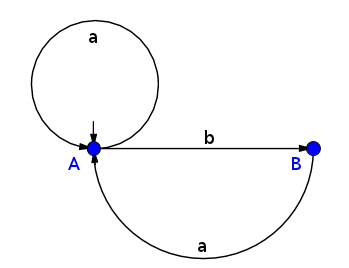
\includegraphics{a.png}}

По $A$ построим однозначную грамматику в соответствии с алгоритмом из теории предыдущих заданий:
\begin{align*}
  S &\rightarrow A \\
  A &\rightarrow \eps | a A | b B \\
  B &\rightarrow \eps | a A
\end{align*}

Преобразуем ее праволинейную:
\begin{align*}
  S &\rightarrow A | \eps \\
  A &\rightarrow a A | a | b B | b \\
  B &\rightarrow a A | a
\end{align*}

Составим СОУ:

$$
\begin{cases}
  S = A + \eps \\
  A = a A + a + b B + b \\
  B = a A + a
\end{cases}
$$

Составим систему линейных уравнений:

$$
\begin{cases}
  S[t] = A[t] + 1 \\
  A[t] = t A[t] + t + t B[t] + t \\
  B[t] = t A[t] + t
\end{cases}
$$

Выразим $S[t]$:

$$
  S[t] = \frac{t + 1}{1 - t - t^2} = - \frac{1 + t}{(t - \frac{-1 - \sqrt{5}}{2}) (t - \frac{-1 + \sqrt{5}}{2})}
$$

Разложим на простые дроби:

$$
  S[t] = \frac{\frac{1 - \sqrt{5}}{2 \sqrt{5}}}{t - \frac{-1 - \sqrt{5}}{2}} -
   \frac{\frac{1 + \sqrt{5}}{2 \sqrt{5}}}{t - \frac{-1 + \sqrt{5}}{2}}
$$

Преобразуем:

$$
  S[t] = -\frac{\frac{\sqrt{5} (1 - \sqrt{5})^2}{20}}{1 - \frac{1 - \sqrt{5}}{2} t} +
   \frac{\frac{\sqrt{5} (1 + \sqrt{5})^2}{20}}{1 - \frac{1 + \sqrt{5}}{2} t}
$$

При разложении в ряд коэффициент $s_n$ при $t^n$ будет:

$$
  s_n = -\frac{\sqrt{5} (1 - \sqrt{5})^2}{20} {\left( \frac{1 - \sqrt{5}}{2} \right)}^n +
   \frac{\sqrt{5} (1 + \sqrt{5})^2}{20} {\left( \frac{1 + \sqrt{5}}{2} \right)}^n
$$

Преобразуем:

$$
  s_n = \frac{{\left( \frac{1 + \sqrt{5}}{2} \right)}^{n + 2} - {\left( \frac{1 - \sqrt{5}}{2} \right)}^{n + 2}}{\sqrt{5}}
$$

\medskip

{\bf Задача 4}

Составим таблицу соответствия символов слова $w = 010$ номерам ячеек ленты для записи конфигураций.

\smallskip

\centerline{
  \begin{tabular}{|c||c|c|c|}
    \hline                       
    символ слова & 0 & 1 & 0 \\
    \hline
    номер ячейки & 1 & 2 & 3 \\
    \hline  
  \end{tabular}
}

\smallskip

{\bf (iii)}
Слово $w = 010$ принимается, принимающее вычисление:

$$
  (q_0, 1) \vdash (q_1, 2) \vdash (q_2, 3) \vdash (q_2, 4)
$$

\smallskip

{\bf (i)}
Как видно из пункта $(iii)$ состояние $q_{t=010}$, в которое автомат в первый раз выходит из префикса $t = 010$ есть $q_2$.

\smallskip

{\bf (ii)}
Построим $\tau_{t = 010}$.
\begin{align*}
  (q_0, 3) &\vdash (q_1, 4) \\
  (q_1, 3) &\vdash (q_0, 2) \vdash (q_1, 3) \vdash ... \\
  (q_2, 3) &\vdash (q_2, 4)
\end{align*}

Получаем $\tau_{t = 010} = (q_0, q_1), (q_1, \star), (q_2, q_2)$.


\end{document}
